\chapter[RESULTS AND DISCUSSION]{Results and Discussion}\label{ch:IV}

\section{Application Features}\label{sec:4.1}

\subsection{Location Search}\label{sec:4.1.1}

The application enables users to search for specific destinations within the
building by providing an origin and a destination. This feature serves as the
primary entry point for route generation. Figure~\ref{fig:4.1} shows the
location search feature.

\begin{figure}[htbp]
\centering

\includegraphics[width=\linewidth]{figures/fig-4-1.png}
\caption{Location search}\label{fig:4.1}
\end{figure}

\subsection{Multiple Floor Support}\label{sec:4.1.2}

The application supports the viewing of buildings with multiple floors, allows
users to navigate between the different floor levels, and provides the option to
select different wings for each floor. Figure~\ref{fig:4.2} displays the options
for the user to select from specific areas of the building.

\begin{figure}[htbp]
\centering
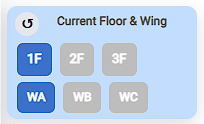
\includegraphics[width=2.60in]{figures/fig-4-2.png}
\caption{Floor and wing selector}\label{fig:4.2}
\end{figure}

\subsection{Map Visualization}\label{sec:4.1.3}

The application provides an interactive indoor map that allows users to zoom,
pan, and reset the viewing area. Figures~\ref{fig:4.3} and~\ref{fig:4.4} show
the 2D floor view and the 3D visualization when navigating.

\begin{figure}[htbp]
\centering
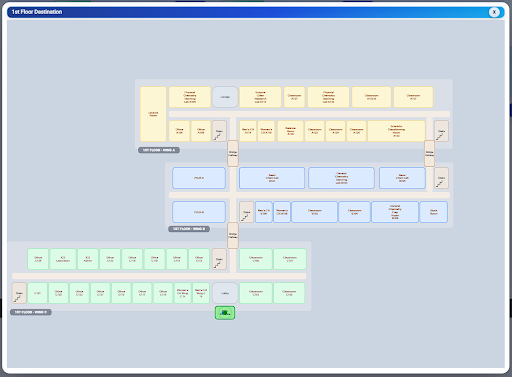
\includegraphics[width=5.20in]{figures/fig-4-3.png}
\caption{Two-dimensional (2D) map view}\label{fig:4.3}
\end{figure}

\begin{figure}[htbp]
\centering
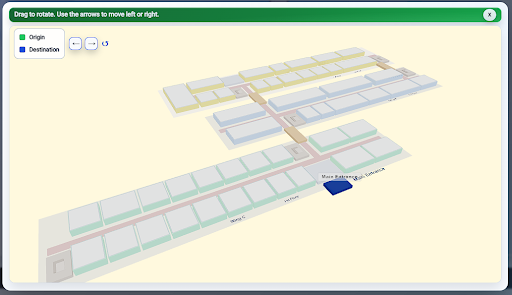
\includegraphics[width=5.20in]{figures/fig-4-4.png}
\caption{Three-dimensional (3D) map view}\label{fig:4.4}
\end{figure}

\subsection{Multi-Floor Layout Builder}\label{sec:4.1.4}

The application includes a layout builder that enables administrators to create
and edit an indoor map to be seen by the users. Figure~\ref{fig:4.5} shows the
panel for the layout builder, which includes the options available to the
administrator.

\begin{figure}[htbp]
\centering

\includegraphics[width=\linewidth]{figures/fig-4-5.png}
\caption{Layout builder panel}\label{fig:4.5}
\end{figure}

\subsection{Layout Builder Map Drafts}\label{sec:4.1.5}

The application allows administrators to save, load, rename, and delete draft
map versions. Figures~\ref{fig:4.6} and~\ref{fig:4.7} show the Map Layouts and
Map Drafts modals, which allow the administrator to select between map versions.

\begin{figure}[htbp]
\centering
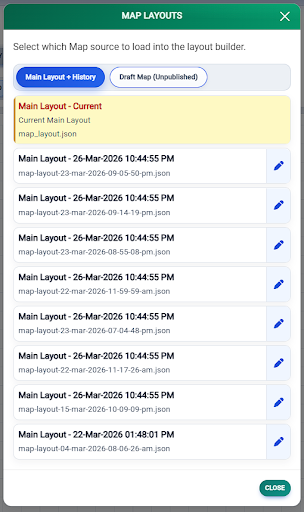
\includegraphics[width=3.00in]{figures/fig-4-6.png}
\caption{Main map layouts}\label{fig:4.6}
\end{figure}

\begin{figure}[htbp]
\centering
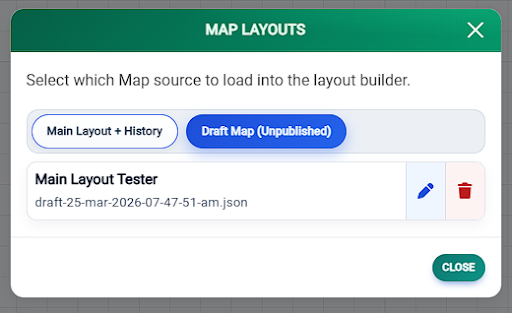
\includegraphics[width=4.60in]{figures/fig-4-7.png}
\caption{Map draft layouts}\label{fig:4.7}
\end{figure}

\subsection{Sandbox Mode}\label{sec:4.1.6}

The application includes a sandbox mode in which administrators can explore the
features of the map layout builder without the risk of overwriting the main map
edits and the published map being displayed to the users. Figure~\ref{fig:4.8}
shows the sandbox mode.

\begin{figure}[htbp]
\centering

\includegraphics[width=5.20in]{figures/fig-4-8.png}
\caption{Sandbox mode}\label{fig:4.8}
\end{figure}

\subsection{Auto-Generated Layouts}\label{sec:4.1.7}

The application has an auto-generate map feature that allows the administrator
to select a set of predefined layouts to assist them with map creation, as shown
in Figure~\ref{fig:4.9}.

\begin{figure}[htbp]
\centering
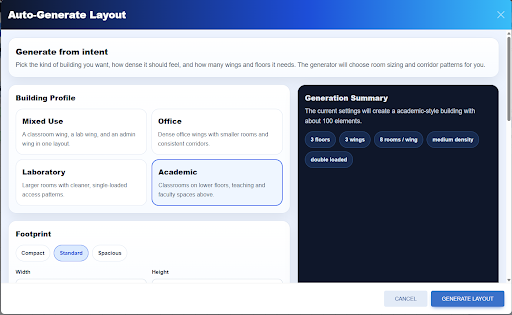
\includegraphics[width=5.20in]{figures/fig-4-9.png}
\caption{Auto-generate map layout}\label{fig:4.9}
\end{figure}

\section{Types of Users}\label{sec:4.2}

The application recognizes two types of users:

\textbf{Admin.} Administrators can modify the mapping of the building, manage
location data, and update floor plans.

\textbf{User.} Users can search for locations within the building and use the
navigation features to access floors, rooms, and routes.

\section{Mapping of the Floor Layout}\label{sec:4.3}

The floor layout of the building is developed through the application's layout
builder, where the admin creates and organizes the map structure for each floor.
The admin directly encodes the building layout within the web application.

Using the layout builder, the admin defines the major spaces of the building,
such as rooms, hallways, stairs, bridges, and entrances. In this process, each
floor is treated as a two-dimensional plane with \emph{x} and \emph{y}
coordinates, allowing the admin to position each component based on its \emph{x}
and \emph{y} location and to size it according to its width and height within
the floor plane. Labels are assigned so that the digital floor plan reflects the
actual arrangement of the building.

The admin can revise the floor plan during the mapping process, and draft
versions of the layout can be created and edited before publication. Once the
admin finalizes the layout, the floor plan is published and becomes the
reference used for navigation display within the application. Previously
published versions of a map can also be reverted to and saved as a new draft,
allowing the admin to roll back changes when needed.

After the map is published, the application uses the mapped structure and
computes the navigation routing based on the details provided by each component
to determine the path from one point to another, as described in the next
section.

\section{Route Computation}\label{sec:4.4}

PathFinder computes routes with the A* search algorithm, the same algorithm used
by Google Maps~\cite{ref06} and by the campus locator map of Ramos et
al.~\cite{ref10}. The search runs on a navigation graph that the backend builds
from the published layout.

\textbf{Navigation graph.} Each room, door, hallway segment, stairway, and the
main entrance becomes a node positioned at its \emph{x} and \emph{y} coordinates
on its floor. Edges join consecutive hallway segments along each corridor;
connect each room, through a door node placed on the room wall facing the
corridor, to the nearest suitable hallway on the same floor; connect each
stairway to a hallway on its floor and to the stairways directly above and below
it; and link the wings through the bridges. An edge is not added when the
straight segment between its two nodes would cut through the interior of another
room. Because building the graph is computationally expensive, the result is
stored in the navigation\_graph\_caches table and reused until a different
layout is published.

\textbf{Edge cost.} The cost of moving between two connected nodes \emph{u} and
\emph{v} is

\begin{equation}
\label{eq:4.1}
c(u,v) = d(u,v) + 150|f_{u} - f_{v}| + p_{J}(u,v) + p_{D}(u,v)
\end{equation}

\noindent where \emph{d}(\emph{u}, \emph{v}) is the straight-line distance
between the two nodes on the floor plane, in layout coordinate units (for a
hallway, measured to the nearest point of its rectangle);
\emph{f}\textsubscript{u} and \emph{f}\textsubscript{v} are the floor numbers of
the two nodes; \emph{p}\textsubscript{J}(\emph{u}, \emph{v}) is 120 when both
nodes are room-connection junctions, 24 when only one of them is, and 0
otherwise; and \emph{p}\textsubscript{D}(\emph{u}, \emph{v}) is 25 when both
nodes are doors and 0 otherwise. The floor term discourages unnecessary floor
changes, while the junction and door terms keep routes on the main hallways
instead of passing from one room entrance to the next.

\textbf{Search.} A* repeatedly expands the unexplored node with the lowest
estimated total cost

\begin{equation}
\label{eq:4.2}
f(n) = g(n) + h(n)
\end{equation}

\noindent where \emph{g}(\emph{n}) is the lowest known cost from the origin to
node \emph{n} computed with Equation~\ref{eq:4.1}, and the heuristic
\emph{h}(\emph{n}) is the straight-line distance from \emph{n} to the
destination. The search skips any edge that crosses the interior of a room not
marked as passable, so a route never cuts through a room.

\textbf{Routes between wings.} When the origin and destination are in different
wings, the route must cross one of the bridges that connect Wings A, B, and C.
The backend prepares candidate sequences of bridge waypoints, computes each leg
between consecutive waypoints with the same search but with the heuristic set to
zero, which makes it equivalent to Dijkstra's algorithm, joins the legs, and
keeps the candidate whose drawn route is shortest. When the origin and
destination are on the same floor but the best route leaves that floor, the
route is recomputed with the nodes on other floors excluded. If a route passes
through the door of a room other than the origin or destination, it is
recomputed with that door excluded.

Finally, the route is simplified for display and returned to the frontend as one
Scalable Vector Graphics (SVG) path per floor, which the map view draws as the
route overlay.

\section{Navigation User Interface}\label{sec:4.5}

Users can find specific locations within the building with the search
functionality and select their origin and destination points by typing in the
search bars or by choosing the rooms in the room list selector.
Figures~\ref{fig:4.10} and~\ref{fig:4.11} show the user interface from the
user's perspective, whereas Figure~\ref{fig:4.12} displays the interface from
the administrator's perspective.

\begin{figure}[htbp]
\centering
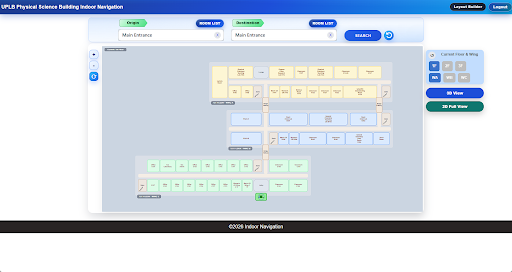
\includegraphics[width=5.40in]{figures/fig-4-10.png}
\caption{Main user interface}\label{fig:4.10}
\end{figure}

\begin{figure}[htbp]
\centering
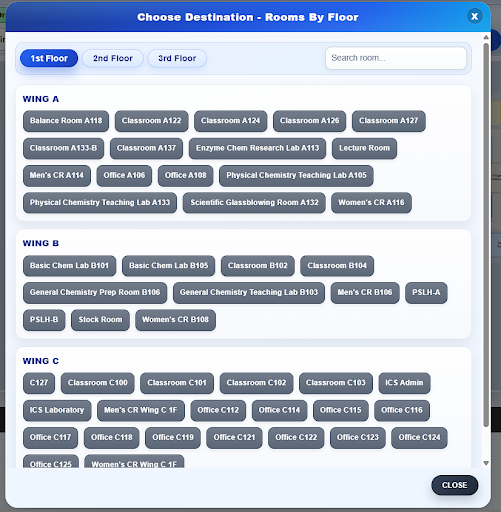
\includegraphics[width=4.20in]{figures/fig-4-11.png}
\caption{Room selector}\label{fig:4.11}
\end{figure}

\begin{figure}[htbp]
\centering
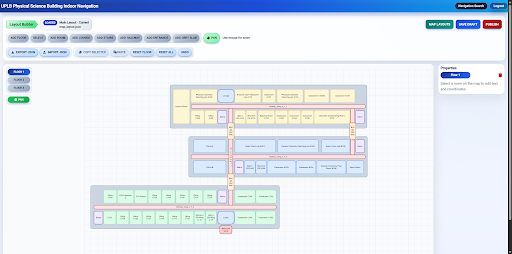
\includegraphics[width=5.40in]{figures/fig-4-12.png}
\caption{Administrator user interface}\label{fig:4.12}
\end{figure}

\section{Non-Functional Requirements}\label{sec:4.6}

\textbf{Usability.} This requirement was met through a guided user interface.
The application provides assisted search suggestions, room-list browsing, clear
map controls, visible route overlays, and consistent navigation elements, making
it easier for users to understand and operate the system.

\textbf{Performance.} This requirement was met by having the application
implemented to be browser-based, which means it can operate and is compatible on
devices capable of running modern web browsers without requiring a
platform-specific installation

\textbf{Scalability.} This requirement was met through the separation of
frontend and backend services, containerized deployment, graph caching, and a
database for storage persistence to accommodate larger map layouts and multiple
maps.

\textbf{Security.} This requirement was met through administrator login,
protected access to the layout builder only for administrators, session
expiration, and controlled Cross-Origin Resource Sharing (CORS) settings.
However, more robust authorization would further improve security.

\textbf{Availability.} This requirement was supported through the application's
AWS-based deployment and service health mechanisms. The system was deployed on
an AWS EC2 instance using Docker containers for both the frontend and backend,
allowing the services to remain isolated and easier to restart when needed.

\section{User Testing Results}\label{sec:4.7}

A total of ten (10) responses were collected, with four coming from building
administrators from UPMO and six from students studying at the University of the
Philippines Los Baños.

\subsection{System Usability Scale}\label{sec:4.7.1}

Table~\ref{tab:4.1} shows the raw questionnaire results from the users, and
Table~\ref{tab:4.2} shows the SUS score of each respondent and the rating to
which the score belongs. The computation of each score using
Equation~\ref{eq:3.1} is shown in Appendix~\ref{app:D}.

\begin{table}[htbp]
\centering
\singlespacing
\caption{Raw SUS responses per respondent}\label{tab:4.1}
\renewcommand{\arraystretch}{1.15}
\begin{tabular}{lcccccccccc}
\toprule
\textbf{Respondent} & \textbf{Q1} & \textbf{Q2} & \textbf{Q3} & \textbf{Q4} & \textbf{Q5} & \textbf{Q6} & \textbf{Q7} & \textbf{Q8} & \textbf{Q9} & \textbf{Q10} \\
\midrule
R1 & 4 & 1 & 5 & 1 & 5 & 3 & 5 & 5 & 5 & 5 \\
R2 & 3 & 1 & 5 & 1 & 4 & 3 & 4 & 1 & 5 & 1 \\
R3 & 4 & 2 & 4 & 2 & 5 & 3 & 5 & 4 & 4 & 4 \\
R4 & 5 & 1 & 5 & 1 & 5 & 1 & 5 & 1 & 5 & 2 \\
R5 & 5 & 1 & 5 & 1 & 5 & 1 & 5 & 1 & 5 & 1 \\
R6 & 3 & 1 & 4 & 3 & 4 & 1 & 4 & 2 & 4 & 5 \\
\bottomrule
\end{tabular}
\par\vspace{4pt}
{\footnotesize\raggedright\setlength{\parindent}{0pt}Responses range from 1 (Strongly disagree) to 5 (Strongly agree).\par}
\end{table}

\begin{table}[htbp]
\centering
\singlespacing
\caption{SUS score, grade, and rating per respondent}\label{tab:4.2}
\renewcommand{\arraystretch}{1.15}
\begin{tabular}{lcl}
\toprule
\textbf{Respondent} & \textbf{SUS Score} & \textbf{Rating} \\
\midrule
R1 & 72.5 & Good \\
R2 & 85.0 & Excellent \\
R3 & 67.5 & OK \\
R4 & 97.5 & Excellent \\
R5 & 100.0 & Excellent \\
R6 & 67.5 & OK \\
Mean & 81.67 & Excellent \\
Median & 78.75 & Good \\
\bottomrule
\end{tabular}
\par\vspace{4pt}
{\footnotesize\raggedright\setlength{\parindent}{0pt}Grades and ratings follow Table~\ref{tab:3.3}.\par}
\end{table}

The six end users who completed the system usability questionnaire produced
individual scores of 72.5, 85.0, 67.5, 97.5, 100.0, and 67.5, for a mean of
81.67 and a median of 78.75. The mean score of 81.67 falls within the
``Excellent'' range of the scale in Table~\ref{tab:3.3}, indicating strong
overall satisfaction with the navigation experience. Three respondents gave
scores in the ``Excellent'' range, while two respondents scored at the lower end
(67.5, rated ``OK''), suggesting that while the majority found the system highly
usable, a subset encountered enough friction to rate the experience more
moderately.

\subsection{Navigation Accuracy}\label{sec:4.7.2}

Qualitatively, all six student respondents confirmed that the application
successfully led them to their intended destination and described the routes as
accurate or mostly accurate. Two respondents noted that routes involving
stairways were occasionally not the shortest or most efficient option available,
and another respondent recommended that the system be tested against a wider
variety of stairway configurations. Respondents highlighted the
three-dimensional view as an effective way to visualize paths across multiple
floors compared to the two-dimensional view. Clarity in routing was rated
favorably, with respondents describing the interface as straightforward and
simple to understand.

\subsection{Layout Builder Evaluation}\label{sec:4.7.3}

The four building administrators who tested the layout builder feature described
the tool as generally intuitive and responsive, and useful for early-stage
planning of floor layouts. Respondents pointed out that the interface was
straightforward to navigate and use, and that the resulting layouts helped
communicate proposed arrangements to clients. One respondent noted that the
application functioned effectively like a bubble diagram, a tool used for
visualizing room connections before a final layout is committed. One feature
identified for improvement was the addition of an autosave function; respondents
mentioned that accidental misclicks could cause unsaved progress to be lost.
Administrator respondents also pointed out that they had difficulty
distinguishing the purpose of the Layout Builder from the Sandbox mode, which
added complexity to understanding the separation between the two functions.
